\documentclass[12pt]{beamer}
\usepackage{listings}
\usepackage[]{color}
\usepackage{bbding}
\usepackage{ragged2e}
\usepackage{tikz}
\usetikzlibrary{decorations.pathreplacing}

\beamertemplatenavigationsymbolsempty
\AtBeginSection[]
{
    \begin{frame}
    \frametitle{Table of Contents}
    \tableofcontents[currentsection]
    \end{frame}
}
\setlength{\tabcolsep}{10pt}
\newcommand{\bigoh}[1]{\mathcal{O}\left(#1\right)}
\newcommand{\TLE}{\textcolor{blue}{TLE}}
\newcommand{\WA}{\textcolor{red}{WA}}
\newcommand{\MLE}{\textcolor{orange}{MLE}}
\newcommand{\AC}{\textcolor{green}{AC}}
\newcommand{\blank}{\vspace{.5cm}}

\definecolor{mygreen}{rgb}{0,0.6,0}
\definecolor{mygray}{rgb}{0.5,0.5,0.5}
\definecolor{mymauve}{rgb}{0.58,0,0.82}

\lstset{ %
  backgroundcolor=\color{white},   % choose the background color; you must add \usepackage{color} or \usepackage{xcolor}
  basicstyle=\tiny,        % the size of the fonts that are used for the code
  breakatwhitespace=false,         % sets if automatic breaks should only happen at whitespace
  breaklines=true,                 % sets automatic line breaking
  commentstyle=\color{mygreen},    % comment style
  deletekeywords={...},            % if you want to delete keywords from the given language
  escapeinside={\%*}{*)},          % if you want to add LaTeX within your code
  extendedchars=true,              % lets you use non-ASCII characters; for 8-bits encodings only, does not work with UTF-8
  frame=single,                    % adds a frame around the code
  keepspaces=true,                 % keeps spaces in text, useful for keeping indentation of code (possibly needs columns=flexible)
  keywordstyle=\color{blue},       % keyword style
  language=C++,                 % the language of the code
  morekeywords={*,...},            % if you want to add more keywords to the set
  numbers=left,                    % where to put the line-numbers; possible values are (none, left, right)
  numbersep=5pt,                   % how far the line-numbers are from the code
  numberstyle=\tiny\color{mygray}, % the style that is used for the line-numbers
  rulecolor=\color{black},         % if not set, the frame-color may be changed on line-breaks within not-black text (e.g. comments (green here))
  showspaces=false,                % show spaces everywhere adding particular underscores; it overrides 'showstringspaces'
  showstringspaces=false,          % underline spaces within strings only
  showtabs=false,                  % show tabs within strings adding particular underscores
  stepnumber=1,                    % the step between two line-numbers. If it's 1, each line will be numbered
  stringstyle=\color{mymauve},     % string literal style
  tabsize=2                      % sets default tabsize to 2 spaces
}

\title{Dynamic Programming I}
\subtitle{Top-Down, Bottom-Up and Classical Problems}
\author{beOI Training \\\tiny{(many thanks to Fran\c{c}ois Aubry)}}
\institute{
\includegraphics[height=12em]{../shared-img/beoi-logo}}

\begin{document}

\frame{\titlepage}

\section{Motivating Problem I: Partition Problem}

\begin{frame}
    \frametitle{Let's start with an example}
    \textbf{Partition Problem}: \\\blank
    Given a set of $n \leq 50$ goodies each with value $v[i] \leq 10$, is it possible to divide them between $3$ persons evenly? 

\end{frame}

\begin{frame}
    \frametitle{Strategy}
    Put yourself in the shoes of the one who divides the goodies.
    \begin{center}
        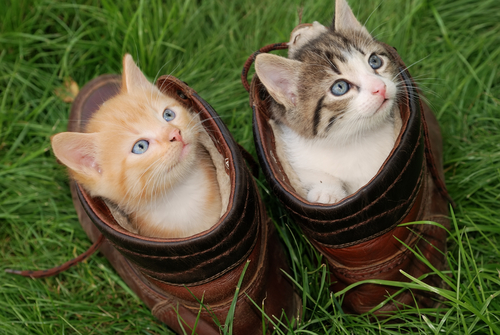
\includegraphics[scale=.75]{img/shoes.jpg}
    \end{center}

    For each goodie, what \textbf{choices} can you make? \pause

    \begin{center}
        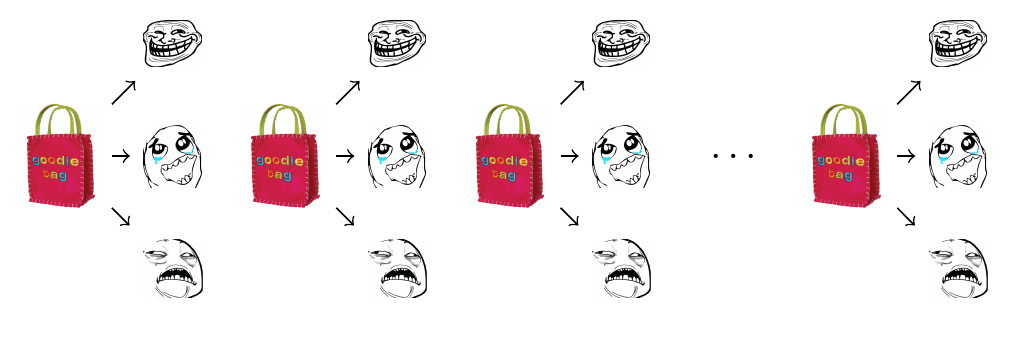
\includegraphics[scale=.3]{img/choices.png}
    \end{center}
\end{frame}

\begin{frame}
    \frametitle{Brute-Force?}
    Suppose we make a brute force algorithm that tries all choices. 
    \\\blank
    What should we keep track of? \pause \\\blank
    \begin{enumerate}
        \item The items we considered so far. \\\blank
            Does the order in which we consider the items matter? \pause \textbf{No}. \\\blank
            $ \Rightarrow $ Just keep an integer $i$ such that we have made choices for items $< i$. \pause \\\blank
        \item At the end we need to know if the division is fair. Do we need to know the items given to each person? \pause \textbf{No}. \\\blank
            $ \Rightarrow $ Just keep track of how much was given to each person.
    \end{enumerate}
\end{frame}

\begin{frame}
    \frametitle{Brute-Force solution}
    \lstinputlisting{listings/brute-force.cpp}
    \pause
    Complexity? \pause $\bigoh{3^n}$ \TLE \\\blank
    We can do better\ldots
\end{frame}

\begin{frame}
    \frametitle{State space and state graph}
    We call one tuple $ (i, given1, given2, given3) $ a \textbf{state}. \\\blank
    We can now define the \textbf{state graph}: its vertices are the states, and there is an edge from $s_1$ to $s_2$ if $s_1$ calls $s_2$ recursively. \\\blank
    How many nodes does the state graph of the previous algorithm have? \\\blank
    $ \bigoh{n \cdot S^3} $ where $S$ is the sum of the goodie values. \\\blank
    But the algorithm is $\bigoh{3^n}$. What's going on? \pause \\\blank
    \textbf{Each state is visited several times $\Rightarrow$ waste of time!}
\end{frame}

\begin{frame}
    What we want to do is to traverse the state graph (DFS like). \\\blank
    How can we achieve that? \pause
    \lstinputlisting{listings/partition-problem.cpp} \pause \blank
    Is this enough to get \AC? \pause \textbf{No}. \\
    The graph has $ \approx n \cdot S^3 = 50 \cdot 500^3 = 6250000000$ nodes $\Rightarrow$ \MLE.
\end{frame}

\begin{frame}
    \begin{center}
        
\includegraphics[scale=.4]{img/sad.jpg}
    \end{center}
    Or can we make it work?
\end{frame}

\begin{frame}
    \frametitle{State space reduction}
    Observe that at the end $ given3 = S - given1 - given2 $. \\\blank
    Thus we can drop one parameter and reduce the state space to $ n \cdot S^2 $.
    \lstinputlisting{listings/partition-problem-better.cpp} \blank
    This is called \textbf{State space reduction}
\end{frame}

\begin{frame}
    \frametitle{What we learned so far}
    \begin{enumerate}
        \item View the problem as a \textbf{sequence of choices}. \blank
        \item Represent the problem with the smallest state space possible. \blank
        \item Perform a DFS on the state graph (remembering visited states). 
    \end{enumerate}
    \pause \blank
    Let's see another example!
\end{frame}

\section{Motivating Problem II: Knapsack Problem}

\begin{frame}
    \frametitle{Knapsack Problem}
    Given a set of $n$ objects each with value $v[i]$ and weight $w[i]$, and a knapsack that can hold a total capacity of $C$. \\\blank
    Choose a subset of objects that fits into the knapsack and has maximum total value. \\\blank
    \flushright
    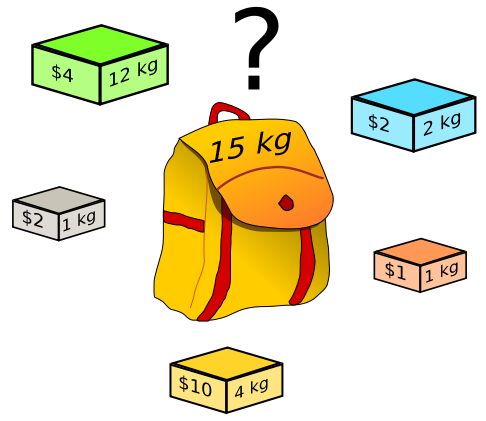
\includegraphics[scale=.2]{img/knapsack.png}
\end{frame}

\begin{frame}
    In what way is this problem similar to the previous one? \pause \\\blank
    \begin{itemize}
        \item Succession of choices: for each item, take it or leave it. \blank
        \item Order does not matter. \blank
    \end{itemize}
    State space? \pause $(i, wtaken)$ \\\blank
    \begin{itemize}
        \item $i = \textit{item we are considering}$
        \item $wtaken = \textit{total weight of the items we selected so far}$
    \end{itemize}
    \blank
    Size of the state space? \pause $\bigoh{n \cdot C}$
\end{frame}

\begin{frame}
    Successors of state $(i, wtaken)$? \pause
    \begin{center}
        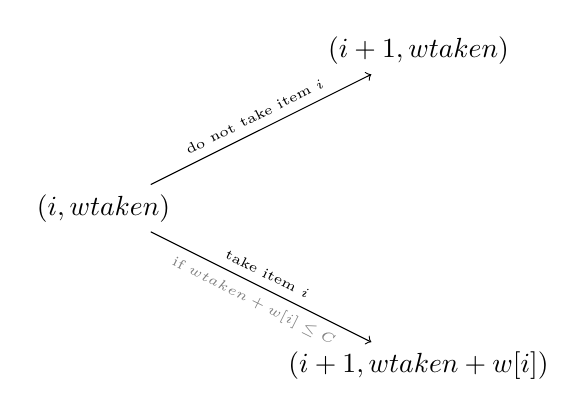
\begin{tikzpicture}
            \node (a) at (0, 0) {$(i, wtaken)$};
            \node (b) at (4, 2) {$(i + 1, wtaken)$};
            \node (c) at (4, -2) {$(i + 1, wtaken + w[i])$};
            \draw[->] (a) edge[midway, pos=0.5, sloped, above] node {\tiny do not take item $i$} (b);
            \draw[->] (a) edge node[midway, pos=0.5, sloped, above] {\tiny take item $i$} node[midway, pos=0.5, sloped, below, gray] {\tiny if $wtaken + w[i] \leq C$} (c);
        \end{tikzpicture}
    \end{center}
\end{frame}

\begin{frame}
    Recurrence relation? \pause
    \[ f(i, wtaken) = \max \Big( f(i+1, wtaken), v[i] + f(i+1, wtaken+w[i]) \Big) \]
    Beware of the knapsack constraint! If $wtaken > C$, the knapsack has no value.
    \[ wtaken > C \Rightarrow f(i, wtaken) = -\infty \]
\end{frame}

\begin{frame}
    \frametitle{Knapsack solution}
    \lstinputlisting{listings/knapsack.cpp}
\end{frame}

\begin{frame}
    Example of a Knapsack state space.
    \begin{center}
        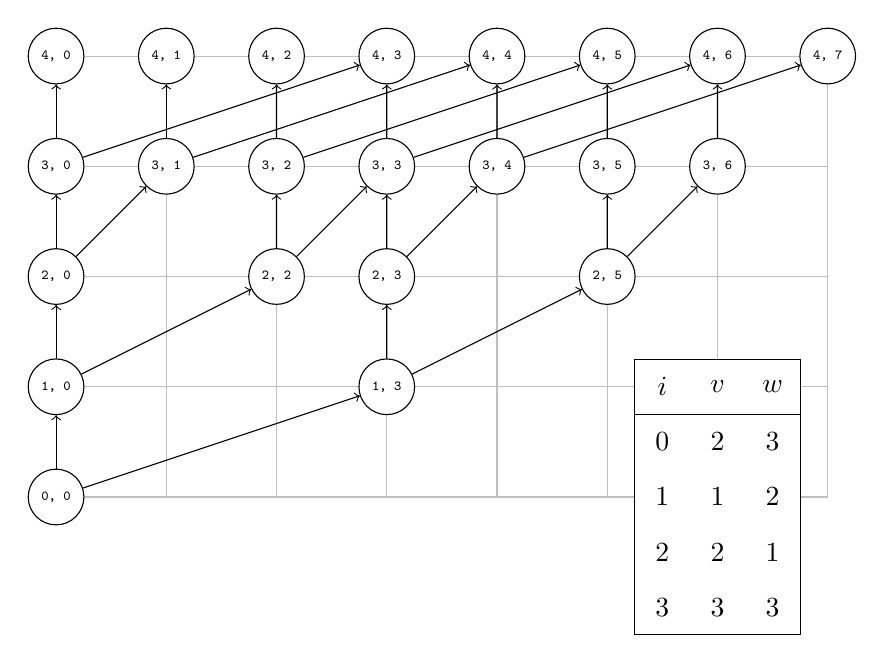
\begin{tikzpicture}[scale=.7]
            \draw[step=2,gray!50!white] (0, 0) grid (14,8);

            \node[draw, fill = white, circle] (00) at (0, 0) {\tiny \texttt{0, 0}};
            \node[draw, fill = white, circle] (10) at (0, 2) {\tiny \texttt{1, 0}};
            \node[draw, fill = white, circle] (20) at (0, 4) {\tiny \texttt{2, 0}};
            \node[draw, fill = white, circle] (30) at (0, 6) {\tiny \texttt{3, 0}};
            \node[draw, fill = white, circle] (40) at (0, 8) {\tiny \texttt{4, 0}};

            \node[draw, fill = white, circle] (31) at (2, 6) {\tiny \texttt{3, 1}};
            \node[draw, fill = white, circle] (41) at (2, 8) {\tiny \texttt{4, 1}};

            \node[draw, fill = white, circle] (22) at (4, 4) {\tiny \texttt{2, 2}};
            \node[draw, fill = white, circle] (32) at (4, 6) {\tiny \texttt{3, 2}};
            \node[draw, fill = white, circle] (42) at (4, 8) {\tiny \texttt{4, 2}};

            \node[draw, fill = white, circle] (13) at (6, 2) {\tiny \texttt{1, 3}};
            \node[draw, fill = white, circle] (23) at (6, 4) {\tiny \texttt{2, 3}};
            \node[draw, fill = white, circle] (33) at (6, 6) {\tiny \texttt{3, 3}};
            \node[draw, fill = white, circle] (43) at (6, 8) {\tiny \texttt{4, 3}};

            \node[draw, fill = white, circle] (34) at (8, 6) {\tiny \texttt{3, 4}};
            \node[draw, fill = white, circle] (44) at (8, 8) {\tiny \texttt{4, 4}};

            \node[draw, fill = white, circle] (25) at (10, 4) {\tiny \texttt{2, 5}};
            \node[draw, fill = white, circle] (35) at (10, 6) {\tiny \texttt{3, 5}};
            \node[draw, fill = white, circle] (45) at (10, 8) {\tiny \texttt{4, 5}};

            \node[draw, fill = white, circle] (36) at (12, 6) {\tiny \texttt{3, 6}};
            \node[draw, fill = white, circle] (46) at (12, 8) {\tiny \texttt{4, 6}};

            \node[draw, fill = white, circle] (47) at (14, 8) {\tiny \texttt{4, 7}};

            \draw[->] (00) -- (10);
            \draw[->] (00) -- (13);
            \draw[->] (10) -- (20);
            \draw[->] (20) -- (30);
            \draw[->] (30) -- (40);
            \draw[->] (20) -- (31);
            \draw[->] (31) -- (41);
            \draw[->] (30) -- (43);
            \draw[->] (31) -- (44);
            \draw[->] (10) -- (22);
            \draw[->] (22) -- (32);
            \draw[->] (32) -- (42);
            \draw[->] (22) -- (33);
            \draw[->] (33) -- (43);
            \draw[->] (13) -- (23);
            \draw[->] (23) -- (33);
            \draw[->] (23) -- (34);
            \draw[->] (34) -- (44);
            \draw[->] (32) -- (45);
            \draw[->] (33) -- (46);
            \draw[->] (34) -- (47);
            \draw[->] (13) -- (25);
            \draw[->] (25) -- (35);
            \draw[->] (25) -- (36);
            \draw[->] (35) -- (45);
            \draw[->] (36) -- (46);

            \draw[fill = white] (10.5, -2.5) rectangle (13.5, 2.5);

            \node at (11, 2) {$i$};
            \node at (12, 2) {$v$};
            \node at (13, 2) {$w$};


            \draw (10.5, 1.5) -- (13.5, 1.5);

            \node at (11, 1) {0};
            \node at (12, 1) {2};
            \node at (13, 1) {3};

            \node at (11, 0) {1};
            \node at (12, 0) {1};
            \node at (13, 0) {2};

            \node at (11, -1) {2};
            \node at (12, -1) {2};
            \node at (13, -1) {1};

            \node at (11, -2) {3};
            \node at (12, -2) {3};
            \node at (13, -2) {3};

        \end{tikzpicture}
    \end{center}
\end{frame}

\begin{frame}
    \frametitle{Memory optimization}
    Observe that we don't need all the entries from the \texttt{memo} table. \\\blank
    Sometimes the table is too big and causes \MLE. \\\blank
    In this situation an alternative is to use a \texttt{HashMap} (or \texttt{unordered\_map}). \\\blank
    This way we only use the memory we need.
\end{frame}

\begin{frame}
    \frametitle{Another approach}
    This is one view of Dynamic Programming. Usually refered to as \textbf{memoization}. \\\blank
    Another view is to decompose the problem into \textbf{sub-problems}. \\\blank
    Define an order on the sub-problems: The bigger the harder. \\\blank
    Express the solution of large sub-problems as a function of smaller sub-problems. \\\blank
    Solve from smaller to larger using the function.
\end{frame}

\begin{frame}
    \frametitle{Let's redo the Knapsack this way}
    Decomposition into sub-problems:
    \begin{align*}
        best[i][c] = & \ \text{best way to take objects $0,1,\cdots,i$} \\
        & \ \text{on a knapsack of capacity $c$}
    \end{align*}
    Observe that the real problem we want to solve is $best[n-1][C]$. \\\blank
    The idea is that maybe $best[i][c]$ relates to $best[i-1][c']$.
\end{frame}

\begin{frame}
    \frametitle{Case 1: item $i$ \textbf{does not} belong to Knapsack}
    Suppose we know \textbf{*magically*} that item $i$ \textbf{does not belong} to the optimal solution of $best[i][c]$. \\\blank
    Then we \textbf{forget} about $i$ and take items $0,1,\cdots,i-1$ in the best possible way in the same knapsack. \\\blank
    That is, $best[i][c] = best[i-1][c]$.
\end{frame}

\begin{frame}
    \frametitle{Case 2: item $i$ \textbf{does} belong to Knapsack}
    But what if item $i$ belongs to the optimal solution of $best[i][c]$? \\\blank
    In this case we simply start by putting item $i$ into the knapsack. \\\blank
    Then we put items $0,1,\cdots,i-1$ in the best possible way in a new knapsack of capacity $c - w[i]$. \\\blank
    Thus, $best[i][c] = v[i] + best[i-1][c-w[i]]$. 
\end{frame}

\begin{frame}
    \begin{center}
        
\includegraphics[scale=.4]{img/but.jpg}
    \end{center} \pause
    Well\ldots who cares? We know that item $i$ either is or isn't in the knapsack. \\\blank
    So\ldots just take the best of the two possibilities!
    \[
        best[i][c] = \max \left( best[i-1][c], v[i] + best[i-1][c-w[i]] \right)
    \]
    \\\blank
    Note that $best[i-1][c-w[i]]$ might not be defined if $c < w[i]$.
\end{frame}

\begin{frame}
    It remains to solve the easiest sub-problems, when $i=0$. \pause \\\blank
    \begin{align*}
        best[0][c] = v[&0] \quad \text{if $c \geq w[0]$} \\
        &0 \ \quad \text{otherwise}
    \end{align*}
\end{frame}

\begin{frame}
    \frametitle{It all comes down to graphs}
    We can also think about sub-problems as nodes in a graph. \\\blank
    The edges link sub-problems as nodes in a graph. \\\blank
    \begin{center}
        \begin{tikzpicture}
            \node[fill = white] (a) at (0, 0) {\tiny \texttt{i, c}};
            \node[fill = white] (b) at (0, -2) {\tiny \texttt{i - 1, c}};
            \node[fill = white] (c) at (-4, -2) {\tiny \texttt{i - 1, c - w[i]}};
            \draw[->] (b) -- (a);
            \draw[->] (c) -- (a);
        \end{tikzpicture}
    \end{center}
    \blank
    We need to solve the sob-problems in a \textbf{topological order} of this graph. \\\blank
    $best[i-1][c]$ and $best[i-1][c-w[i]]$ need to be solved before $best[i][c]$.
\end{frame}

\begin{frame}
    \frametitle{Implementation}
    \lstinputlisting{listings/knapsack-bottom-up.cpp}
    \blank
    For most DP problems, a topological order can be achieved simply with the proper sequencing of some (nested) loops.
\end{frame}

\section{Top-Down and Bottom-Up}

\begin{frame}
    \frametitle{Two approaches}
    The first approach starts from the hardest sub-problem (the pair $(0, 0)$) and breaks it down into easier sub-problems. \\\blank
    We call that a \textbf{Top-Down DP}. \\\blank
    The second approach starts from the easy sub-problems and builds up harder sub-problems upon it. \\\blank
    We call that a \textbf{Bottom-Up DP} \\\blank
    Generally, Top-Down is implemented \textbf{recursively} and Bottom-Up \textbf{iteratively}. \\\blank
    How do you know which one you should use?
\end{frame}

\begin{frame}
    \frametitle{Top-Down DP vs Bottom-Up DP}
    Top-Down: \\\blank
    \textbf{+} Only computes relevant states. \\\blank
    \textbf{+} Easier to come up with. \\\blank
    Bottom-Up: \\\blank
    \textbf{+} Usually possible to reduce the memory. \\\blank
    \PencilRightDown Implement Knapsack with $\bigoh{C}$ memory. \\\blank
    \textbf{--} Solves all sub-problems.
\end{frame}

\section{Guided Exercise}

\begin{frame}
    \frametitle{Let's solve a problem together}
    \centering
    \Huge{UVa 562: Dividing coins}
\end{frame}

\section{Motivating Problem III: Shortest Path Problem}

\begin{frame}
    \frametitle{Shortest path problem}
    Given a directed, weighted graph $G$ and a vertex $s$, compute the length of the shortest path from $s$ to all other vertices. \\\blank
    Let's solve this problem using \textbf{DP}. \\\blank
    What could be our sub-problems?
\end{frame}

\begin{frame}
    Let's try
    \[
        sp[v] = \text{length of the shortest path from $s$ to $v$}
    \]
    \blank
    How does $sp[v]$ relate with other problems? \pause
    \[ 
        sp[s] = 0
    \]
    \[
        sp[v] = \min_{u \in \delta^-(v)} sp[u] + w(u, v)
    \]
    where $\delta^-(u)$ is the set of in-neighbours of $v$.

    \begin{center}
        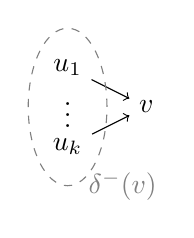
\begin{tikzpicture}[scale = 0.5]
            \node (v) at (0, 0) {$v$};
            \node (u1) at (-2, 1) {$u_1$};
            \node at (-2, 0) {$\vdots$};
            \node (uk) at (-2, -1) {$u_k$};
            \draw[->] (u1) -- (v);
            \draw[->] (uk) -- (v);
            \draw[dashed, gray] (-2, 0) ellipse (1cm and 2cm);
            \node[gray] at (-0.6, -2) {$\delta^-(v)$};
        \end{tikzpicture}
    \end{center}

    Does this work? \textbf{No!} \pause \\
    \begin{tikzpicture}[overlay]
        \node at  (9, 2) {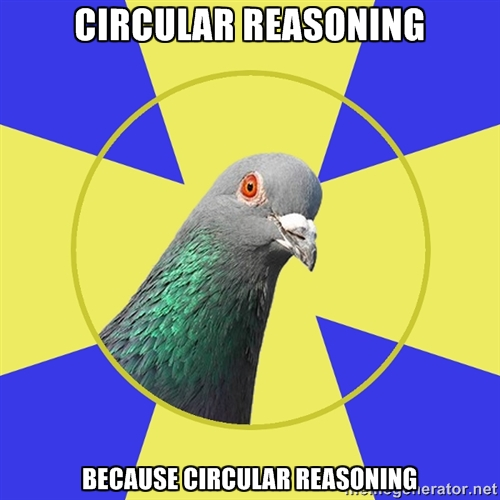
\includegraphics[scale = 0.3]{img/circular.jpg}};
    \end{tikzpicture}

\end{frame}

\begin{frame}
    If $v$ belongs to a \textbf{cycle}, $sp[v]$ depends on $sp[v]$\ldots \\\blank
    For \textbf{DP} to work, we need the underlying sub-problem graph to be \textbf{acyclic}. \\\blank
    Observe that the \textbf{sub-problem} graph is actually\ldots the input graph $G$. \\\blank
    The above recurrence works for acyclic graphs.

\end{frame}

\begin{frame}
    \frametitle{Shortest path for acyclic graphs}
    \[ sp[v] = \text{length of the shortest path from $s$ to $v$} \]
    \[ sp[s] = 0 \]
    \[ sp[v] = \min_{u \in \delta^-(v)} sp[u] + w(u, v) \quad \forall v \in V \setminus \{s\} \]
    \blank
    In what order should we compute the problems? \pause\\\blank
    We must have computed $sp[u]$ for all $u \in \delta^-(v)$ before we compute $sp[v]$. \\\blank
    $\Rightarrow$ we need to do it in the \textbf{topological order} of $G$. \pause \\\blank
    That is not surprising, we said we \textbf{always} evaluate DP states in the topological order of the sub-problem graph. \\
    And in this case it is $G$.
\end{frame}

\begin{frame}
    \frametitle{Sub-problem graph must be acyclic}
    This just to say that \\\blank
    \textbf{DP only works if your state space is acyclic!} \\\blank
    Be careful defining your state space.
\end{frame}

\end{document}
